\documentclass{article}

\setlength{\headsep}{0.75 in}
\setlength{\parindent}{0 in}
\setlength{\parskip}{0.1 in}

%=====================================================
% Add PACKAGES Here (You typically would not need to):
%=====================================================

\usepackage{xcolor}
\usepackage[margin=1in]{geometry}
\usepackage{amsmath,amsthm}
\usepackage{fancyhdr}
\usepackage{enumitem}
\usepackage{graphicx}
\usepackage{amsmath, amssymb}  % Include the amsmath and amssymb packages for mathematical symbols

%=====================================================
% Ignore This Part (But Do NOT Delete It:)
%=====================================================

\theoremstyle{definition}
\newtheorem{problem}{Problem}
\newtheorem*{fun}{Fun with Algorithms}
\newtheorem*{challenge}{Challenge Yourself}
\def\fline{\rule{0.75\linewidth}{0.5pt}}
\newcommand{\finishline}{\begin{center}\fline\end{center}}
\newtheorem*{solution*}{Solution}
\newenvironment{solution}{\begin{solution*}}{{\finishline} \end{solution*}}
\newcommand{\grade}[1]{\hfill{\textbf{($\mathbf{#1}$ points)}}}
\newcommand{\thisdate}{April 11, 2024}
\newcommand{\thissemester}{\textbf{Rutgers: Spring 2024}}
\newcommand{\thiscourse}{ECE 509: Convex Optimization} 
\newcommand{\thishomework}{Number} 
\newcommand{\thisname}{Name} 
\newcommand{\thisextension}{Yes/No} 

\headheight 40pt              
\headsep 10pt
\renewcommand{\headrulewidth}{0pt}
\pagestyle{fancy}

\newcommand{\thisheading}{
   \noindent
   \begin{center}
   \framebox{
      \vbox{\vspace{2mm}
    \hbox to 6.28in { \textbf{\thiscourse \hfill \thissemester} }
       \vspace{4mm}
       \hbox to 6.28in { {\Large \hfill Homework \#\thishomework \hfill} }
       \vspace{2mm}
         \hbox to 6.28in { { \hfill \thisdate  \hfill} }
       \vspace{2mm}
       \hbox to 6.28in { \emph{Name: \thisname \hfill Extension: \thisextension}}
      \vspace{2mm}}
      }
   \end{center}
   \bigskip
}

%=====================================================
% Some useful MACROS (you can define your own in the same exact way also)
%=====================================================


\newcommand{\ceil}[1]{{\left\lceil{#1}\right\rceil}}
\newcommand{\floor}[1]{{\left\lfloor{#1}\right\rfloor}}
\newcommand{\prob}[1]{\Pr\paren{#1}}
\newcommand{\expect}[1]{\Exp\bracket{#1}}
\newcommand{\var}[1]{\textnormal{Var}\bracket{#1}}
\newcommand{\set}[1]{\ensuremath{\left\{ #1 \right\}}}
\newcommand{\poly}{\mbox{\rm poly}}


%=====================================================
% Fill Out This Part With Your Own Information:
%=====================================================


\renewcommand{\thishomework}{7} %Homework number
\renewcommand{\thisname}{Ravi Raghavan} % Enter your name here
\renewcommand{\thisextension}{No} % Pick only one of the two options accordingly

\begin{document}

\thisheading
\vspace{-0.75cm}


%=====================================================
% LaTeX Tip: You can erase this part from here.... 
%=====================================================		

\finishline

%=====================================================
% LaTeX Tip: ... to here
%=====================================================	


\bigskip
\begin{problem}
    \textit{Voronoi description of halfspace.} Let $a$ and $b$ be distinct points in $\mathbb{R}^n$. Show that the set of all points that are closer (in Euclidean norm) to $a$ than $b$, \textit{i.e.}, $\{x : ||x - a||_2 \leq  ||x - b||_2 \}$, is a halfspace. Describe it explicitly as an inequality of the form $c^Tx \leq d$. Draw a picture.

    \begin{solution}
        We can see that the following two sets are equivalent: 

        $S_1 = S_2$ where $S_1 = \{x : ||x - a||_2 \leq  ||x - b||_2 \}$ and $S_2 = \{x : ||x - a||^2_2 \leq  ||x - b||^2_2 \}$ \newline 

        Let's work with $S_2$ since it will be a lot easier 

        $S_2 = \{x : ||x - a||^2_2 \leq  ||x - b||^2_2 \}$ \newline 
        $S_2 = \{x : ||x||^2_2 - 2 <x, a> + ||a||^2_2 \leq  ||x||^2_2 - 2<x, b> + ||b||^2_2 \}$ \newline 
        $S_2 = \{x : - 2 <x, a> + ||a||^2_2 \leq  - 2<x, b> + ||b||^2_2 \}$ \newline 
        $S_2 = \{x : 2 <x, b - a> \enspace  \leq  ||b||^2_2 - ||a||^2_2 \}$ \newline 
        $S_2 = \{x : 2 (b - a)^T x \enspace  \leq  ||b||^2_2 - ||a||^2_2 \}$ \newline 
        $S_2 = \{x : (b - a)^T x \enspace  \leq  0.5 (||b||^2_2 - ||a||^2_2) \}$ \newline 

        If we set $c = b - a$ and $d = 0.5 (||b||^2_2 - ||a||^2_2)$, we can express $S_2$ as follows: \newline 
        $S_2 = \{x : c^T x \enspace  \leq d \}$ \newline 
        This is a closed half-space

        \begin{figure}[h!]
        \centering
        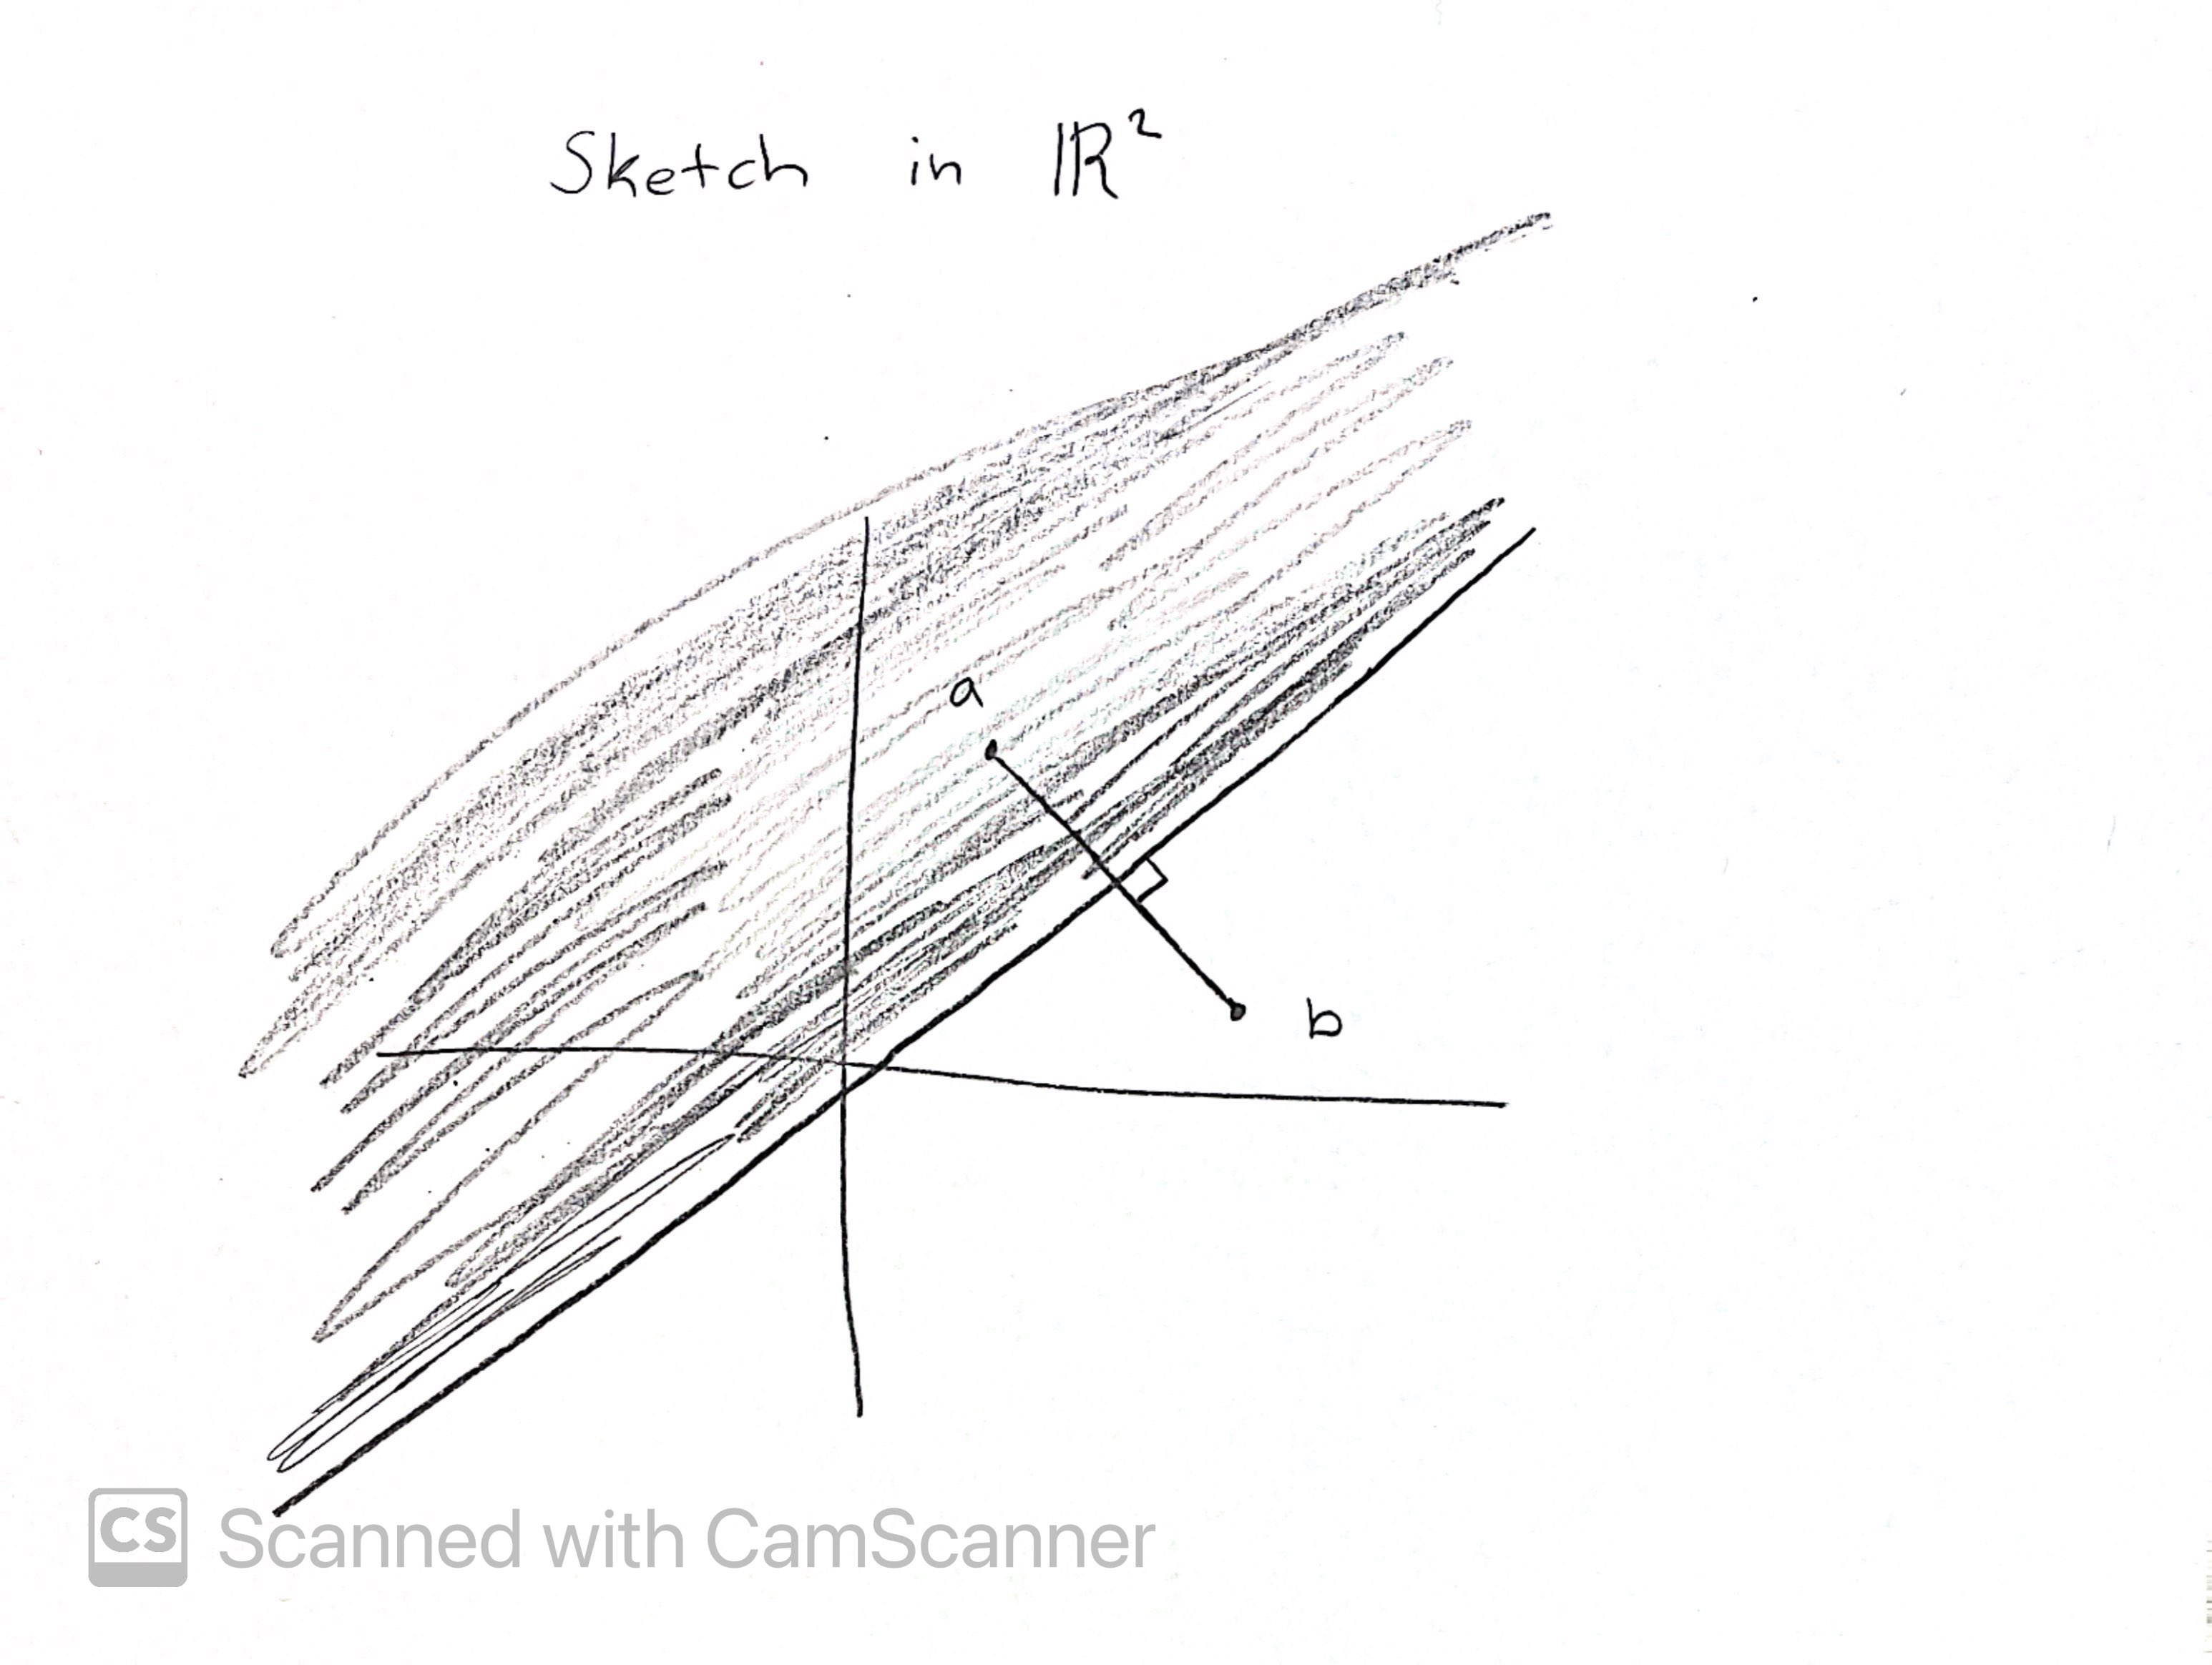
\includegraphics[width=0.6 \textwidth]{Sketchn_1.jpg}
        \caption{Set of Points Closer to $a$ than $b$ in $\mathbb{R}^2$}
    \end{figure}  
        
    \end{solution}
\end{problem}
\newpage 
\begin{problem}
    Which of the following sets $S$ are polyhedra? If possible, express $S$ in the form $S = \{x | Ax \preceq b, Fx = g \}$
\begin{enumerate}
    \item[(b)]  Yes $S$ is a polyhedra. 

    Let $M_1 = [a_1, a_2, ..., a_n] \in \mathbb{R}^{1 x n}$ and let $M_2 = [a_1^2, a_2^2, ..., a_n^2] \in \mathbb{R}^{1 x n}$

    Let $F$ be the vertical concatentation of $1^T$, $M_1$, and $M_2$. Let $g$ be $[1, b_1, b_2]^T$

    Let $A = -I$
    
    We can express $S$, via compact notation, as $S = \{x | Ax \preceq 0, Fx = g \}$

    Note: Just to confirm, $\preceq$ when applied to 2 vectors means component-wise $\leq$

    \item [(c)] $S$ is NOT a Polyhedra. Let's analyze why this is the case. 

    First we must look at the statement $x^Ty \leq 1$ for all $||y||_2 = 1$. Our goal is to take all these inequalities and express them in the form $Ax \preceq b$, where $A$ is a matrix, $\preceq$ when applied to 2 vectors means component-wise $\leq$, and $b$ is a vector. So, given a $y$ where $||y||_2 = 1$, we can put this $y$ in a row of $A$. $Ax \preceq 1$, where each row of $A$ is a feasible value of $y$, would capture the statement $x^Ty \leq 1$ for all $||y||_2 = 1$. 
    
    However, the number of vectors $y$ where $||y||_2 = 1$ is infinite. Hence, our matrix $A$ would have to have infinite rows which is clearly not possible. 

    Another way of looking at it is like this: \newline 
    $S$ is the intersection of an infinite number of halfspaces. As per definition, polyhedra are the intersection of a FINITE number of halfspaces. 
    
    We have proved why $S$ is NOT a polyhedra.  
\end{enumerate}
\end{problem}

\begin{problem}
    \textit{Hyperbolic sets.} Show that the \textit{hyperbolic set} is $\{x \in \mathbb{R}^2_+ : x_1x_2 \geq 1\}$ is convex. As a generalization, show that $\{x \in \mathbb{R}^2_+ : \prod_{i=1}^{n} x_i \geq 1\}$ is convex. \textit{Hint.} If $a, b \geq 0$ and $0 \leq \theta \leq 1$, then $a^{\theta} b^{1 - \theta} \leq \theta a + (1 - \theta) b$

    \begin{solution}

    Let's start by proving that the \textit{hyperbolic set} is $S = \{x \in \mathbb{R}^2_+ : x_1x_2 \geq 1\}$ is convex. \newline 
Let's have two vectors  $j$ and $k$ that are in $S$. Let the elements of $j$ be $j_1, j_2$. Let the elements of $k$ be $k_1, k_2$

We want to prove that $\theta j + (1 - \theta)k \in S$. 

        Since we know that $j \in S$ and $k \in S$, we can state the following:
        \begin{itemize}
            \item $j_1 \geq 0, j_2 \geq 0$
            \item $j_1 j_2 \geq 1$
            \item $k_1 \geq 0, k_2 \geq 0$
            \item $k_1 k_2 \geq 1$
        \end{itemize}

    For $0 \leq \theta \leq 1$, since $j_1 \geq 0, j_2 \geq 0$ and $k_1 \geq 0, k_2 \geq 0$, we can see that $0 \leq j_1^{\theta} k_1^{1 - \theta} \leq \theta j_1 + (1 - \theta)k_1$ and $0 \leq j_2^{\theta} k_2^{1 - \theta} \leq \theta j_2 + (1 - \theta)k_2$. 

    $j_1^{\theta} k_1^{1 - \theta} j_2^{\theta} k_2^{1 - \theta} = (j_1 j_2)^{\theta} (k_1 k_2)^{1 - \theta} $

    Since $j_1 j_2 \geq 1$ and $k_1 k_2 \geq 1$, we can say that: \newline 

    $j_1^{\theta} k_1^{1 - \theta} j_2^{\theta} k_2^{1 - \theta} = (j_1 j_2)^{\theta} (k_1 k_2)^{1 - \theta} \geq 1$

    Since $j_1^{\theta} k_1^{1 - \theta} \leq \theta j_1 + (1 - \theta)k_1$ and $j_2^{\theta} k_2^{1 - \theta} \leq \theta j_2 + (1 - \theta)k_2$

    $1 \leq j_1^{\theta} k_1^{1 - \theta} j_2^{\theta} k_2^{1 - \theta} \leq (\theta j_1 + (1 - \theta)k_1) (\theta j_2 + (1 - \theta)k_2)$

    Furthermore, since $j_1 \geq 0, j_2 \geq 0$ and $k_1 \geq 0, k_2 \geq 0$, we know that $\theta j_1 + (1 - \theta)k_1 \geq 0$ and $\theta j_2 + (1 - \theta)k_2 \geq 0$

    We have finished proving that $\theta j + (1 - \theta)k \in S$. 
    
    Let $S$ be $\{x \in \mathbb{R}^2_+ : \prod_{i=1}^{n} x_i \geq 1\}$. Let's have two vectors  $j$ and $k$ that are in $S$. Let the elements of $j$ be $j_1, j_2, ...., j_n$. Let the elements of $k$ be $k_1, k_2, ..., k_n$

        We want to prove that $\theta j + (1 - \theta)k \in S$. 

        Since we know that $j \in S$ and $k \in S$, we can state the following:
        \begin{itemize}
            \item $j_1 \geq 0, j_2 \geq 0, ...., j_n \geq 0$
            \item $j_1 j_2 j_3 ... j_n \geq 1$
            \item $k_1 \geq 0, k_2 \geq 0, ...., k_n \geq 0$
            \item $k_1 k_2 k_3 ... k_n \geq 1$
        \end{itemize}

        For $i \in [1, n]$, $j_i, k_i \geq 0$ and $0 \leq \theta \leq 1$, we can see that $0 \leq j_i^{\theta} k_i^{1 - \theta} \leq \theta j_i + (1 - \theta)k_i$. 

        We can also see that: \newline 
        
        $\prod_{i=1}^{n} j_i^{\theta} k_i^{1 - \theta} =  (\prod_{i=1}^{n} j_i)^{\theta} (\prod_{i=1}^{n} k_i)^{1 - \theta}$

        Since $j_1 j_2 j_3 ... j_n \geq 1$ and $k_1 k_2 k_3 ... k_n \geq 1$, we can say that: \newline 
        
        $\prod_{i=1}^{n} j_i^{\theta} k_i^{1 - \theta} =  (\prod_{i=1}^{n} j_i)^{\theta} (\prod_{i=1}^{n} k_i)^{1 - \theta} \geq 1$

        Since $j_i^{\theta} k_i^{1 - \theta} \leq \theta j_i + (1 - \theta)k_i$, \newline
        
        $1 \leq \prod_{i=1}^{n} j_i^{\theta} k_i^{1 - \theta} \leq   \prod_{i=1}^{n} \theta j_i + (1 - \theta)k_i$

        Furthermore, since $j_1 \geq 0, j_2 \geq 0, ...., j_n \geq 0$ and $k_1 \geq 0, k_2 \geq 0, ...., k_n \geq 0$, we know that $\theta j_i + (1 - \theta)k_i \geq 0$ as well. 

        We have shown that $\theta j_i + (1 - \theta)k_i \in S$ and that $S$ is a convex set!
        
    \end{solution}
\end{problem}

\begin{problem}
Problem 2.16: \newline 
    Show that if $S_1$ and $S_2$ are convex sets in $\mathbb{R}^{m + n}$, then so is their partial sum \newline 
    $S = \{(x, y_1 + y_2) : x \in \mathbb{R}^m, y_1, y_2 \in \mathbb{R}^n, (x, y_1) \in S_1, (x, y_2) \in S_2 \}$

    \begin{solution}

    Let's say that we have two points in $S$, namely $(x_1, y_{11} + y_{12})$ and $(x_2, y_{21} + y_{22})$. To prove that $S$ is convex, we need to show that $\theta (x_1, y_{11} + y_{12}) + (1 - \theta) (x_2, y_{21} + y_{22})$ is in $S$.  

    Based on the definition of $S$, we can see the following: 
    \begin{itemize}
        \item $(x_1, y_{11}) \in S_1$
        \item $(x_1, y_{12}) \in S_2$
        \item $(x_2, y_{21}) \in S_1$
        \item $(x_2, y_{22}) \in S_2$
    \end{itemize}

    Since $S_1$ and $S_2$ are convex, based on the definition of convex sets, we can see that:
    \begin{itemize}
        \item $\theta (x_1, y_{11}) + (1 - \theta) (x_2, y_{21}) \in S_1$

        $ (\theta x_1 + (1 - \theta) x_2, \theta y_{11} + (1 - \theta) y_{21} ) \in S_1$
        \item $\theta (x_1, y_{12})  + (1 - \theta)(x_2, y_{22}) \in S_2$

        $ (\theta x_1 + (1 - \theta) x_2, \theta y_{12} + (1 - \theta) y_{22} ) \in S_1$
    \end{itemize}

    By definition of Set $S$, since $ (\theta x_1 + (1 - \theta) x_2, \theta y_{11} + (1 - \theta) y_{21} ) \in S_1$ and $ (\theta x_1 + (1 - \theta) x_2, \theta y_{12} + (1 - \theta) y_{22} ) \in S_1$, we can see that: \newline 

    $ (\theta x_1 + (1 - \theta) x_2, (\theta y_{11} + (1 - \theta) y_{21}) + (\theta y_{12} + (1 - \theta) y_{22}) ) \in S$ \newline 

        $ (\theta x_1 + (1 - \theta) x_2, \theta (y_{11} + y_{12}) + (1 - \theta) (y_{21} + y_{22}) ) \in S$ \newline 

$\theta (x_1, y_{11} + y_{12}) + (1 - \theta) (x_2, y_{21} + y_{22})$ is in $S$.  We have proven that $S$ is convex
    
        
    \end{solution}
\end{problem}

\begin{problem} [Problem 2.19(a)]
    \textit{Linear-fractional functions and convex sets.} Let $f: \mathbb{R}^m \rightarrow \mathbb{R}^n$ be the linear-fractional function
    \begin{equation}
        f(x) = (Ax + b) / (c^Tx + d), \enspace dom f = \{x | c^Tx + d > 0\}
    \end{equation}

    In this problem, we study the inverse image of a convex set $C$ under $f$, \textit{i.e.,}
    \begin{equation}
        f^{-1}(C) = \{x \in dom f : f(x) \in C\}
    \end{equation}

    For each of the following sets $C \subseteq \mathbb{R}^n $, give a simple description of $f^{-1}(C)$

    \begin{solution}
        Let's look at the halfspace $C = \{y : g^Ty \leq h\}$(with $g\neq 0$). 

        $f^{-1}(C) = \{x :  g^T ((Ax + b) / (c^Tx + d)) \leq h, c^Tx + d > 0 \}$ \newline 

        Since $c^Tx + d > 0$ \newline 
        $f^{-1}(C) = \{ x :  g^T (Ax + b) \leq h(c^Tx + d), c^Tx + d > 0 \}$ \newline 
        $f^{-1}(C) = \{ x :  g^TAx + g^Tb \leq hc^Tx + hd, c^Tx + d > 0 \}$ \newline
        $f^{-1}(C) = \{ x :  (g^TA - hc^T)x \leq hd - g^Tb, c^Tx + d > 0 \}$ \newline
        $f^{-1}(C) = \{ x :  (A^Tg - ch^T)^T x \leq hd - g^Tb, c^Tx + d > 0 \}$ \newline

        Let's call a new vector $p^T = (A^Tg - ch^T)^T$ and $q = hd - g^Tb$ \newline 
        $f^{-1}(C) = \{ x :  p^T x \leq q, c^Tx + d > 0 \}$ \newline

        We can see that $f^{-1}(C)$ is just the intersection of a halfspace and the domain of f!
    \end{solution}
\end{problem}

\begin{problem} [Problem 3.17]
Suppose $p < 1, p \neq 0$. Show that the function 
\begin{equation}
    f(x) = (\sum_{i=1}^{n} x_i^p)^{\frac{1}{p}}
\end{equation}
with $dom f = \mathbb{R}^n_{++}$ is concave. This includes as special cases $f(x) = (\sum_{i=1}^{n} x_i^2)^{\frac{1}{2}}$ and the \textit{harmonic mean} $f(x) = (\sum_{i=1}^{n} \frac{1}{x_i})^{-1}$. \textit{Hint.} Adapt the proofs for the log-sum-exp
function and the geometric mean in 3.1.5

\begin{solution}
    Gradient: $\frac{\partial{f}}{\partial{x_k}} = (\sum_{i=1}^{n} x_i^p)^{\frac{1}{p} - 1} x_k^{p - 1}$

    Jacobian: \newline 
    $\frac{\partial^2{f}}{\partial^2{x_k}} = (1 - p) (\sum_{i=1}^{n} x_i^p)^{\frac{1}{p} - 2} [x_k^{2p - 2} - x_k^{p - 2} \sum_{i=1}^{n} x_i^p]$ \newline 
    $\frac{\partial^2{f}}{\partial{x_k} \partial{x_l}} = (1 - p) (\sum_{i=1}^{n} x_i^p)^{\frac{1}{p} - 2} x_l^{p - 1} x_k^{p - 1}$ \newline 

    It is clear that we can express $\nabla^2f(x)$ as follows: \newline 
    $\nabla^2f(x) = (1 - p) (\sum_{i=1}^{n} x_i^p)^{\frac{1}{p} - 2} [qq^T - (\sum_{i=1}^{n} x_i^p) diag(x_1^{p - 2}, x_2^{p - 2}, \dots, x_n^{p - 2})]$ where $q_i = x_i^{p - 1}$ \newline 

    For concavity, we need $v^T \nabla^2f(x) v \leq 0$ to hold true for all $x \in \mathbb{R}^n_{++}$

    $v^T \nabla^2f(x) v  = (1 - p) (\sum_{i=1}^{n} x_i^p)^{-\frac{1}{p}} [v^Tqq^Tv (\sum_{i=1}^{n} x_i^p)^{\frac{2}{p} - 2} - (\sum_{i=1}^{n} x_i^p)^{\frac{2}{p} - 1} v^T diag(x_1^{p - 2}, x_2^{p - 2}, \dots, x_n^{p - 2}) v]$

    $v^T \nabla^2f(x) v  = (1 - p) (\sum_{i=1}^{n} x_i^p)^{-\frac{1}{p}} [(\sum_{i=1}^{n} x_i^{p - 1} v_i)^2 ((\sum_{i=1}^{n} x_i^p)^{\frac{1}{p} - 1})^2 - (\sum_{i=1}^{n} x_i^p)^{\frac{2}{p} - 1} v^T diag(x_1^{p - 2}, x_2^{p - 2}, \dots, x_n^{p - 2}) v]$

    $v^T \nabla^2f(x) v  = (1 - p) (\sum_{i=1}^{n} x_i^p)^{-\frac{1}{p}} [(\sum_{i=1}^{n} ((\sum_{i=1}^{n} x_i^p)^{\frac{1}{p} - 1}) x_i^{p - 1} v_i)^2  - \sum_{i=1}^{n} x_i^{p - 2} v_i^2 ((\sum_{i=1}^{n} x_i^p)^{\frac{2}{p} - 1})]$


    The Cauchy Schwartz Inequality tell us that $(a^Ta) (b^Tb) \geq (a^Tb)^2$ \newline 
    If we set $a_i = x_i^{\frac{p}{2}} ((\sum_{i=1}^{n} x_i^p)^{\frac{-1}{2}})$ and we set $b_i = x_i^{\frac{p - 2}{2}} v_i ((\sum_{i=1}^{n} x_i^p)^{\frac{1}{p} - \frac{1}{2}})$, substituting this into the Cauchy Schwartz inequality allows us to see that 

    $(\sum_{i=1}^{n} x_i^p)  ((\sum_{i=1}^{n} x_i^p)^{-1}) (\sum_{i=1}^{n} x_i^{p - 2} v_i) ((\sum_{i=1}^{n} x_i^p)^{\frac{2}{p} - 1}) \geq (\sum_{i = 1}^{n} x_i^{p - 1} v_i )^2 ((\sum_{i=1}^{n} x_i^p)^{\frac{2}{p} - 2})$ \newline 

    Simplication of LHS[Left Hand Side]: \newline 
    $(\sum_{i=1}^{n} x_i^p)  ((\sum_{i=1}^{n} x_i^p)^{-1}) (\sum_{i=1}^{n} x_i^{p - 2} v_i) ((\sum_{i=1}^{n} x_i^p)^{\frac{2}{p} - 1}) = (\sum_{i=1}^{n} x_i^{p - 2} v_i) ((\sum_{i=1}^{n} x_i^p)^{\frac{2}{p} - 1})$ \newline 
    
    $= (\sum_{i=1}^{n} x_i^p)^{\frac{2}{p} - 1} v^T diag(x_1^{p - 2}, x_2^{p - 2}, \dots, x_n^{p - 2}) v$

    Simplication of RHS[Right Hand Side]: \newline 
    $v^Tqq^Tv (\sum_{i=1}^{n} x_i^p)^{\frac{2}{p} - 2}$

    Since LHS $\geq$ RHS, we can state that: \newline 

    $(\sum_{i=1}^{n} x_i^p)^{\frac{2}{p} - 1} v^T diag(x_1^{p - 2}, x_2^{p - 2}, \dots, x_n^{p - 2}) v \geq v^Tqq^Tv (\sum_{i=1}^{n} x_i^p)^{\frac{2}{p} - 2}$

    $v^Tqq^Tv (\sum_{i=1}^{n} x_i^p)^{\frac{2}{p} - 2} - (\sum_{i=1}^{n} x_i^p)^{\frac{2}{p} - 1} v^T diag(x_1^{p - 2}, x_2^{p - 2}, \dots, x_n^{p - 2}) v \leq 0$

    Since $p < 1$ and $x_i \in \mathbb{R}_{++}$, $(1 - p) (\sum_{i=1}^{n} x_i^p)^{\frac{-1}{p}}$ is a positive constant. \newline 

    $v^T \nabla^2f(x) v  = (1 - p) (\sum_{i=1}^{n} x_i^p)^{-\frac{1}{p}} [v^Tqq^Tv (\sum_{i=1}^{n} x_i^p)^{\frac{2}{p} - 2} - (\sum_{i=1}^{n} x_i^p)^{\frac{2}{p} - 1} v^T diag(x_1^{p - 2}, x_2^{p - 2}, \dots, x_n^{p - 2}) v] \leq 0$
    
    Hence, since $v^T \nabla^2f(x) v \leq 0$, we have proven concavity!
    
\end{solution}
\end{problem}

\begin{problem}
    Adapt the proof of concavity of the log-determinant function in §3.1.5 to show the following
    \begin{itemize}
        \item[(a)] $f(X) = tr(X^{-1})$ is convex on $dom f = \mathbb{S}^n_{++}$
        \begin{solution}
            To verify convexity, we can consider an arbitrary line given by $X = Z + tV$ where $Z \in \mathbb{S}^n_{++}$ and $V \in \mathbb{S}^n$

            $g(t) = f(Z + tV) = tr((Z + tV)^{-1})$ \newline 
            $= tr((Z^{\frac{1}{2}} (I + tZ^{\frac{-1}{2}} V Z^{\frac{-1}{2}}) Z^{\frac{1}{2}})^{-1})$ \newline 
            $= tr((Z^{\frac{-1}{2}} (I + tZ^{\frac{-1}{2}} V Z^{\frac{-1}{2}})^{-1} Z^{\frac{-1}{2}}))$ \newline 

            It is a well known fact that $tr(ABC) = tr(BCA) = tr(CAB)$ \newline 

            Hence, we can continue our simplification \newline 
            $= tr((Z^{\frac{-1}{2}} Z^{\frac{-1}{2}} (I + tZ^{\frac{-1}{2}} V Z^{\frac{-1}{2}})^{-1}))$ \newline 

            $= tr((Z^{-1} (I + tZ^{\frac{-1}{2}} V Z^{\frac{-1}{2}})^{-1}))$ \newline 

            Let us represent $Z^{\frac{-1}{2}} V Z^{\frac{-1}{2}}$ as an Eigenvalue Decomposition of $QDQ^T$ \newline 
            
            $= tr((Z^{-1} (I + tQDQ^T)^{-1}))$ \newline 
            $= tr((Z^{-1} (QIQ^T + tQDQ^T)^{-1}))$ \newline 
            $= tr((Z^{-1} (Q(I + tD)Q^T)^{-1}))$ \newline 
            $= tr((Z^{-1} Q (I + tD)^{-1} Q^T))$ \newline 

            Again, we can use the cyclic property of the trace: \newline 
            $= tr((Q^TZ^{-1} Q (I + tD)^{-1}))$ \newline 

            $= \sum_{i=1}^{n} (Q^TZ^{-1} Q)_{ii} (1 + t\lambda_i)^{-1}$

            Note: $\lambda_i$ are eigenvalues of $Z^{\frac{-1}{2}} V Z^{\frac{-1}{2}}$ 

            Since $Z$ is a positive definite, symmetric matrix, we know that $Z^{-1}$ is a positive definite, symmetric matrix as well. Hence, $(Q^TZ^{-1} Q)_{ii}$ is always positive. \newline 

            Let's now look at $(1 + t\lambda_i)^{-1}$. Let's take the second derivative with respect to $t$. This second derivative is equal to $\frac{2\lambda_i^2}{(1 + t\lambda_i)^3}$. The numerator is clearly positive. \newline 

            We know that $Z + tV \in \mathbb{S}^n_{++}$ \newline 
            This means that $Z^{\frac{1}{2}} (I + tZ^{\frac{-1}{2}} V Z^{\frac{-1}{2}}) Z^{\frac{1}{2}} \in \mathbb{S}^n_{++}$ \newline 
            This means that $(I + tZ^{\frac{-1}{2}} V Z^{\frac{-1}{2}}) \in \mathbb{S}^n_{++}$ must be True

            This means that $1 + t\lambda_i > 0$ must be true for all $i$!. Hence, the denominator of $\frac{2\lambda_i^2}{(1 + t\lambda_i)^3}$ is positive as well. 

            We have shown that the second derivative of $(1 + t\lambda_i)^{-1}$ is positive over the values of $t$ that are in the domain of $g$ which means that $(1 + t\lambda_i)^{-1}$ is a convex function over the domain of $g$.

            $\sum_{i=1}^{n} (Q^TZ^{-1} Q)_{ii} (1 + t\lambda_i)^{-1}$ is a non-negative weighted sum of convex functions which is convex!

            We have completed the proof!

        \end{solution}  
    \end{itemize}
\end{problem}

\begin{problem}
    \textit{ Nonnegative weighted sums and integrals}
    \begin{itemize}
        \item[(a)] Show that $f(x) = \sum_{i=1}^{r} \alpha_i x_{[i]}$ is a convex function of $x$, where $\alpha_1 \geq \alpha_2 \geq \dots \alpha_r \geq 0$, and $x_{[i]}$  denotes the $ith$ largest component of $x$. (You can use the fact that $f(x) = \sum_{i=1}^{r}  x_{[i]}$ is convex on $\mathbb{R}^n$)

        \begin{solution}
            $f(x) = \alpha_r (\sum_{i=1}^{r}  x_{[i]}) + (\alpha_{r - 1} - \alpha_r) (\sum_{i=1}^{r - 1}  x_{[i]}) + (\alpha_{r - 2} - \alpha_{r - 1}) (\sum_{i=1}^{r - 2}  x_{[i]}) + \dots + (\alpha_{1} - \alpha_{2}) (x_{[1]})$ 

            Since $a_{i} > a_{i + 1}$, $a_{i} - a_{i + 1} > 0$. \newline 

            We know that a non-negative combination of convex functions is convex. Hence, we have completed the proof
        \end{solution}

        \item[(b)] Let $T(x, w)$  denote the trigonometric polynomial
        \begin{equation}
            T(x, w) = x_1 + x_2 \cos{w} + x_3 \cos{2w} + \dots + x_n \cos{(n - 1)w}
         \end{equation}

         
Show that the function 
\begin{equation}
    f(x) = - \int_{0}^{2\pi} \log T(x, w) \,dw
\end{equation}

is convex on $\{x \in \mathbb{R}^n : T(x, w) > 0, 0 \leq w \leq 2\pi\}$

\begin{solution}
    Let $g(x, w) = - \log T(x, w) = - \log(x_1 + x_2 \cos{w} + x_3 \cos{2w} + \dots + x_n \cos{(n - 1)w})$ \newline 

    Let's prove that $g(x, w)$ is convex in $x$ when we fix $w$ \newline 

    $h(t) = g(z + tv, w) = - \log T(z + tv, w) = - \log(z_1 + tv_1 + (\cos{w})(z_2 + tv_2) +  (\cos{2w}) (z_3 + tv_3) + \dots + (\cos{(n - 1)w}) (z_n + tv_n))$ \newline 

    $h'(t) = - \frac{v_1 + v_2 \cos{w} + v_3 \cos{2w} + \dots + v_n \cos{(n - 1)w} }{T(z + tv, w)}$ \newline 

    $h''(t) = \frac{(v_1 + v_2 \cos{w} + v_3 \cos{2w} + \dots + v_n \cos{(n - 1)w} )^2}{T(z + tv, w)^2} \geq 0$

    This means that $g(x, w)$ is convex for a fixed $w$ \newline 

    Hence, $f(x) = \int_{0}^{2\pi} g(x, w) \,dw$ is like an infinite non-negative weighted sum. Hence, $f(x)$ is convex!
    

\end{solution}
    \end{itemize}
\end{problem}


\end{document}





